\documentclass[a4paper,12pt]{article}   % papír A4, písmo 12 bodu
\usepackage[utf8x]{inputenc}            %kodovaní UTF-8
\usepackage{ucs}                        %kodovani unicode
\usepackage[czech]{babel}               %podpora cestiny
\usepackage[T1]{fontenc}                %pouzij variantu pisma T1 (hacky, carky)
\usepackage[left=2.5cm,right=1.5cm,top=2.5cm,bottom=2.5cm]{geometry} %okraje stranky
\usepackage{amsmath,amsfonts,amssymb}   %podpora matematiky
\usepackage{gensymb,marvosym}           %symboly celsius (\celsius) apod.
%\usepackage{mathptmx}                   %font Times New Roman s~podporou matematiky
\usepackage{times}                      %font Times New Roman (matematika pismem Computer Modern) 
\usepackage{parskip}                    %mezera mezi odstavci
%\usepackage[document]{ragged2e}         %text zarovany vlevo
\usepackage[none]{hyphenat} \sloppy     %slova nedelit a~nepretekat
\usepackage{titlesec}
\setcounter{secnumdepth}{4}
\clubpenalty 10000                      %kontrolovat sirotky
\widowpenalty 10000                     %kontrolovat vdovy
\usepackage{setspace} \onehalfspacing   %podpora pro zmenu radkovani + radkovani 1,5
\usepackage{enumerate}                  %podpora pro zmenu cislovani
\usepackage{parskip}
\usepackage{fancyhdr}                   %vlastni zahlavi a~zapati
\usepackage{graphicx}                   %podpora grafiky
\graphicspath{{materialy/}}                   %vychozi adresar s~obrazky
\usepackage{caption}
\usepackage{subcaption}
\usepackage{siunitx}
\usepackage{MnSymbol,wasysym}
\usepackage[shortlabels]{enumitem}
\usepackage{amsmath}
\usepackage{halloweenmath}

%\usepackage{pgfplots}


%\usepackage[table,xcdraw]{xcolor}

        %%%%%%%--prostredi pro vkladani grafu ---%%%%%%%%%%
\usepackage{float}

\usepackage{url}
\usepackage[unicode]{hyperref}
\usepackage{mhchem}
        %%%%%%%--prostredi pro vkladani grafu ---%%%%%%%%%%

\titleclass{\subsubsubsection}{straight}[\subsection]
\newcounter{subsubsubsection}[subsubsection]
\renewcommand\thesubsubsubsection{\thesubsubsection.\arabic{subsubsubsection}}
\renewcommand\theparagraph{\thesubsubsubsection.\arabic{paragraph}} % optional; useful if paragraphs are to be numbered

\titleformat{\subsubsubsection}
  {\normalfont\normalsize\bfseries}{\thesubsubsubsection}{1em}{}
\titlespacing*{\subsubsubsection}
{0pt}{3.25ex plus 1ex minus .2ex}{1.5ex plus .2ex}

\makeatletter
\renewcommand\paragraph{\@startsection{paragraph}{5}{\z@}%
  {3.25ex \@plus1ex \@minus.2ex}%
  {-1em}%
  {\normalfont\normalsize\bfseries}}
\renewcommand\subparagraph{\@startsection{subparagraph}{6}{\parindent}%
  {3.25ex \@plus1ex \@minus .2ex}%
  {-1em}%
  {\normalfont\normalsize\bfseries}}
\def\toclevel@subsubsubsection{4}
\def\toclevel@paragraph{5}
\def\toclevel@paragraph{6}
\def\l@subsubsubsection{\@dottedtocline{4}{7em}{4em}}
\def\l@paragraph{\@dottedtocline{5}{10em}{5em}}
\def\l@subparagraph{\@dottedtocline{6}{14em}{6em}}
\makeatother

\setcounter{secnumdepth}{4}
\setcounter{tocdepth}{4}
\usepackage{gensymb}

\usepackage{amsmath}

\setlist[enumerate]{itemsep=0mm}


%------------------------------ KONEC PREAMBULE ---------------------------------


\begin{document}
\newfloat{schema}{htbp}{schema}\floatname{schema}{Schéma}
\newfloat{graf}{htbp}{graf}\floatname{graf}{Graf}

\begin{titlepage}


    \begin{center}
        \vspace*{1cm}
            
        \Huge
        \textbf{KMITOČTOVÁ ZÁVISLOST STŘÍDAVÝCH VOLTMETRŮ}
            
        \vspace{0.5cm}
        \LARGE
        
            
        \vspace{1.5cm}
            
        \textbf{Jakub Dvořák}
            
        \vfill
            
        
            
        \vspace{0.8cm}
            
        
            
        \Large
        
        
            
        29.9.2020\\
        \vspace*{.5cm}
        
\includegraphics[width=.4\textwidth]{logo-cvut-fee.png}\\
        
            
    \end{center}
\end{titlepage}

\setcounter{page}{0} %cislo strany
\pagestyle{empty} %stranku necislovat

\newpage
\section{Úkol měření}
\label{zadani}
\begin{enumerate}[label=\alph*)]
    \item V rozsahu kmitočtů 70~Hz až 300~kHz (přibližně v logaritmickém měřítku, tj. pro kmitočty 70, 200, 500~Hz, 1, 3, 10, 20, 50, 100, 200, 300~kHz) změřte kmitočtovou závislost předložených číslicových voltmetrů a~nízkofrekvenčního elektronického voltmetru. Za kmitočtově nezávislý považujte v tomto frekvenčním rozsahu číslicový voltmetr HP~34401A. Měření proveďte na příslušných rozsazích voltmetrů při hodnotách napětí a)~1~V, b)~7~V. Zapojení přístrojů je na schématu~\ref{schema}.
    \item Změřené závislosti vyneste do grafů a~teoreticky zdůvodněte.
\end{enumerate}

\section{Schéma zapojení}
\begin{schema}[h!]
    \centering
    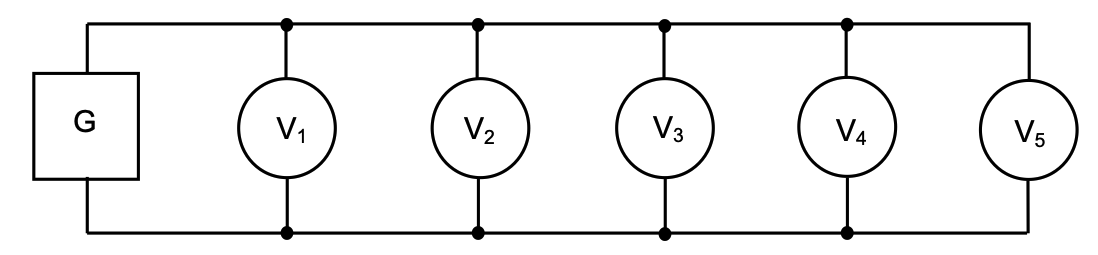
\includegraphics[width=.9\textwidth]{EMB-cv02-schema.png}
    \caption{Zapojení pro měření \cite{protokol}}
    \label{schema}
\end{schema}
\section{Seznam použitých přístrojů}
\begin{itemize}
    \item Frekvenční generátor
    \item Ruční multimetr MY64
    \item Ruční multimetr Summit 45
    \item Stolní multimetr HP 34401 A
    \item Ručičkový multimetr TVT-321
\end{itemize}

\section{Teoretický úvod}
Multimetry jsou základem většiny elektrických měření. Při měření střídavého napětí se způsob jejich měření ale liší. U levnějších přístrojů multimetr střídavý signál usměrní precizním usměrňovačem s operačními zesilovači, aby bylo možné kompenzovat úbytek napětí na diodách. Pro zobrazení \textit{RMS} neboli \textit{střední kvadratické} hodnoty změřenou hodnotu vynásobí koeficientem 1,11. Tento koeficient nicméně platí pouze pro sinusový signál.

U dražších multimetrů se používá tzv. \textit{true RMS converter}, což je dedikovaný obvod, jehož výstup odpovídá \textit{RMS} hodnotě vstupu. Příkladem může být IC AD636 od firmy Analog Devices \cite{datasheet_graf}.

Pro naše měření jsme použili frekvenční generátor generující sinusový průběh. Velikost \textit{střední kvadratické} hodnoty byla na zdroji přesně nastavena podle stolního multimetru HP 34401 A. Ostatní multimetry byly zapojeny paralelně podle schématu~\ref{schema}. 

První měření proběhlo s počátečním $U_{RMS} = 1~\textrm{V}$. Pro druhé měření pak $U_{RMS} = 7~\textrm{V}$. Kmitočty byly nastaveny podle zadání, jak je popsáno v kapitole \ref{zadani}. Při každém kroku frekvence počkáme na ustálení hodnot zobrazovaných multimetrem a~hodnoty odečteme a~zapíšeme.




\section{Zpracování naměřených hodnot}
Naměřená data jsou zobrazena níže v~tabulkách \ref{tab:data1} a~\ref{tab:data2} a~jím odpovídajícím grafům.

\begin{table}[h!]
    \centering
    \begin{tabular}{|c|c|c|c|l|}
    \hline
    \rule{0pt}{2.5ex}MY64 $\frac{U}{V}$&HP 34401 A	$\frac{U}{V}$&Summit 45 $\frac{U}{V}$   &TVT-321 $\frac{U}{V}$   & Frekvence $\frac{f}{Hz}$\\[.7ex]\hline\hline
    0,9870	& 0,9820	& 0,9740	& 0,9700    & 70\\\hline
    0,9900	& 0,9840	& 0,9760	& 0,9750    & 200\\\hline
    0,9880	& 0,9810	& 0,9690	& 0,9700    & 500\\\hline
    0,9890	& 0,9810	& 0,9550	& 0,9700    & 1\,000\\\hline
    0,9870	& 0,9810	& 0,8610	& 0,9700    & 3\,000\\\hline
    0,9550	& 0,9780	& 0,4800	& 0,9620    & 10\,000\\\hline
    0,8960	& 0,9775	& 0,2400	& 0,9600    & 20\,000\\\hline
    0,6990	& 0,9710	& 0,0310	& 0,9600    & 50\,000\\\hline
    0,2700	& 0,9538	& 0,0020	& 0,9200    & 100\,000\\\hline
    0,0030	& 0,9810	& 0,0000	& 0,8790    & 200\,000\\\hline
    0,0030	& 0,8400	& 0,0000	& 0,8200    & 300\,000\\\hline
    \end{tabular}
    \caption{Naměřená data - první měření} 
    \label{tab:data1}
\end{table}

\begin{graf}
    \centering
    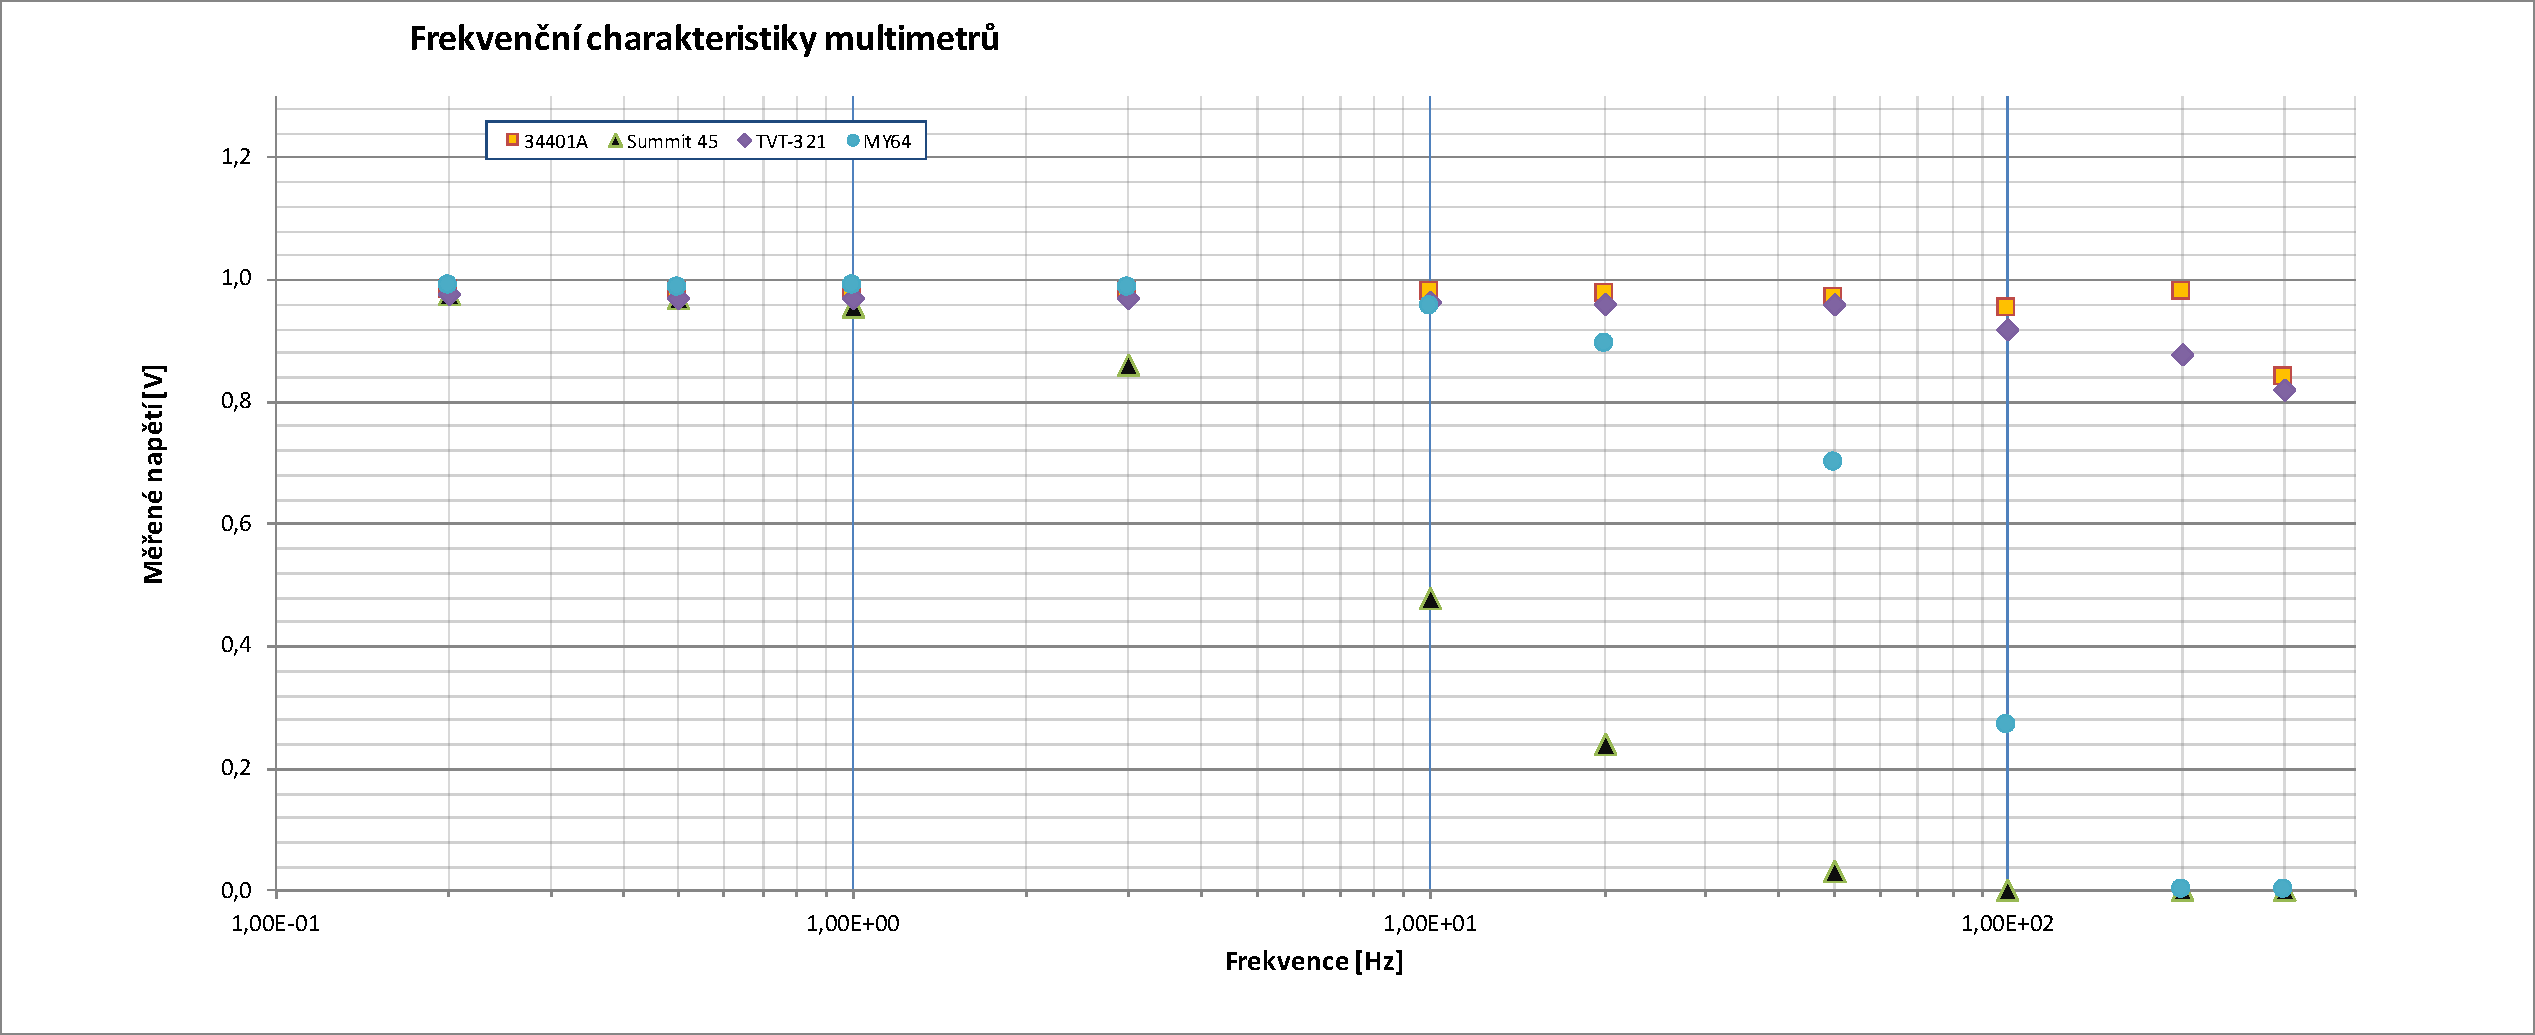
\includegraphics[width=.9\textwidth]{graf1.pdf}
    \caption{Hodnoty z prvního měření}
    \label{graf1}
\end{graf}


\begin{table}[h!]
    \centering
    \begin{tabular}{|c|c|c|c|l|}
    \hline
    \rule{0pt}{2.5ex}MY64 $\frac{U}{V}$&HP 34401 A	$\frac{U}{V}$&Summit 45 $\frac{U}{V}$   &TVT-321 $\frac{U}{V}$   & Frekvence $\frac{f}{Hz}$\\[.7ex]\hline\hline
    7,04	& 7,0014	& 6,89	& 6,9	& 70\\\hline
    7,05	& 7,0209	& 6,91	& 6,9	& 200\\\hline
    7,04	& 7,0159	& 6,90	& 7,0	& 500\\\hline
    7,05	& 7,0209	& 6,88	& 7,0	& 1\,000\\\hline
    7,21	& 7,0101	& 6,80	& 7,0	& 3\,000\\\hline
    9,28	& 6,9876	& 6,54	& 7,0	& 10\,000\\\hline
    14,02	& 6,9818	& 2,03	& 7,2	& 20\,000\\\hline
    18,40	& 6,9285	& 0,92	& 7,4	& 50\,000\\\hline
    21,90	& 6,8136	& 0,50	& 7,4	& 100\,000\\\hline
    4,90	& 6,4430	& 0,08	& 7,1	& 200\,000\\\hline
    0,03	& 5,9160	& 0,01	& 6,7	& 300\,000\\\hline
    \end{tabular}
    \caption{Naměřená data - druhé měření}
    \label{tab:data2}
\end{table}

\begin{graf}
    \centering
    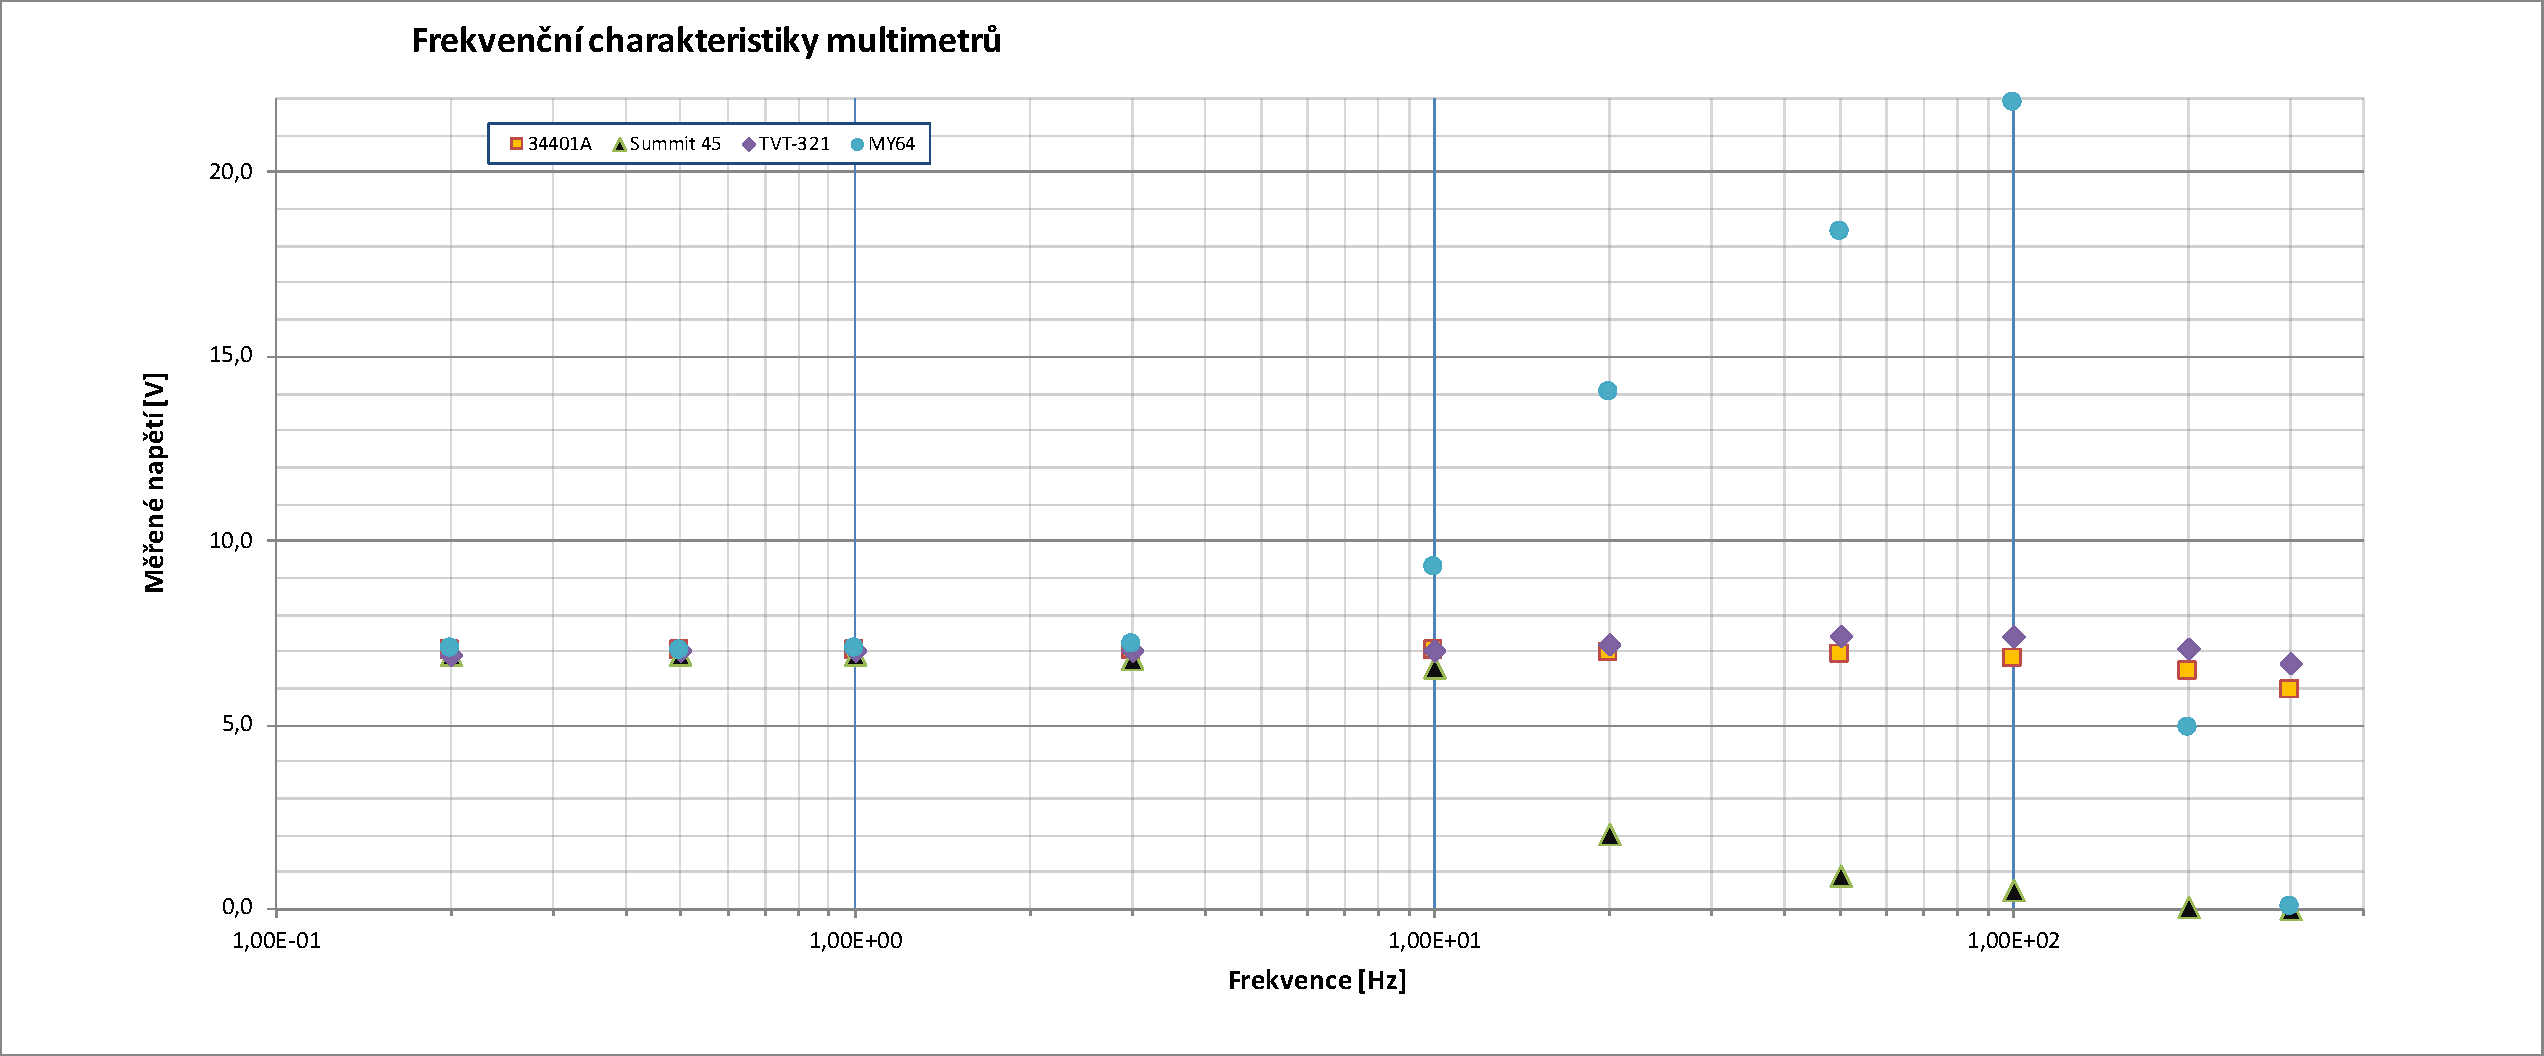
\includegraphics[width=.9\textwidth]{graf2.pdf}
    \caption{Hodnoty z druhého měření}
    \label{graf2}
\end{graf}
\section{Zpracování naměřených dat}
Jak je na první pohled vidět z grafů \ref{graf1} a~\ref{graf2}, tak stejné multimetry se chovaly různě v závislosti na vstupním napětí. Takovéto chování může mít dva důvody. Prvním je frekvenční charakteristika \textit{RMS~převodníku}. Tabulkové závislosti různých vstupních napětí na frekvenci u \textit{RMS~převodníku} AD636 jsou znázorněny v grafu \ref{datasheet}. Pro vyšší hodnoty vstupního napětí se v oblasti $3\cdot10^4 - 3\cdot10^6 \textrm{~Hz}$ objevuje zvýšení výstupního napětí a~až poté následný pokles. Při našem měření se oblast zesílení výstupního napětí objevila mezi frekvencemi $10^4 - 10^5\textrm{~Hz}$. 
Druhým důvodem může být použití přesného usměrňovače a~kondenzátoru paralelně s předřadným odporem. Kondenzátor se zpravidla používá pro zvýšení frekvenčního rozsahu, ale občas dojde k jeho překompenzování a~výsledné napětí se zvýší. 

Multimetr MY64 má podle datasheetu psaný frekvenční rozsah pro měření AC napětí od $40 \textrm{~Hz}$ do~$400\textrm{~Hz}$ a~to s přesností $\pm(0,8\textrm{~\%~of~rdg~}+~3\textrm{~dgt})$. Tedy psaný frekvenční rozsah platí. Pro multimetr Summit~45 je psaný frekvenční rozsah pro měření AC napětí od $45 \textrm{~Hz}$ do~$450\textrm{~Hz}$ a~přesnost je stejná jako u MY64~\cite{datasheet_multimetry}. Naměřené hodnoty odpovídají tabulkové přesnosti.

\begin{graf}
    \centering
    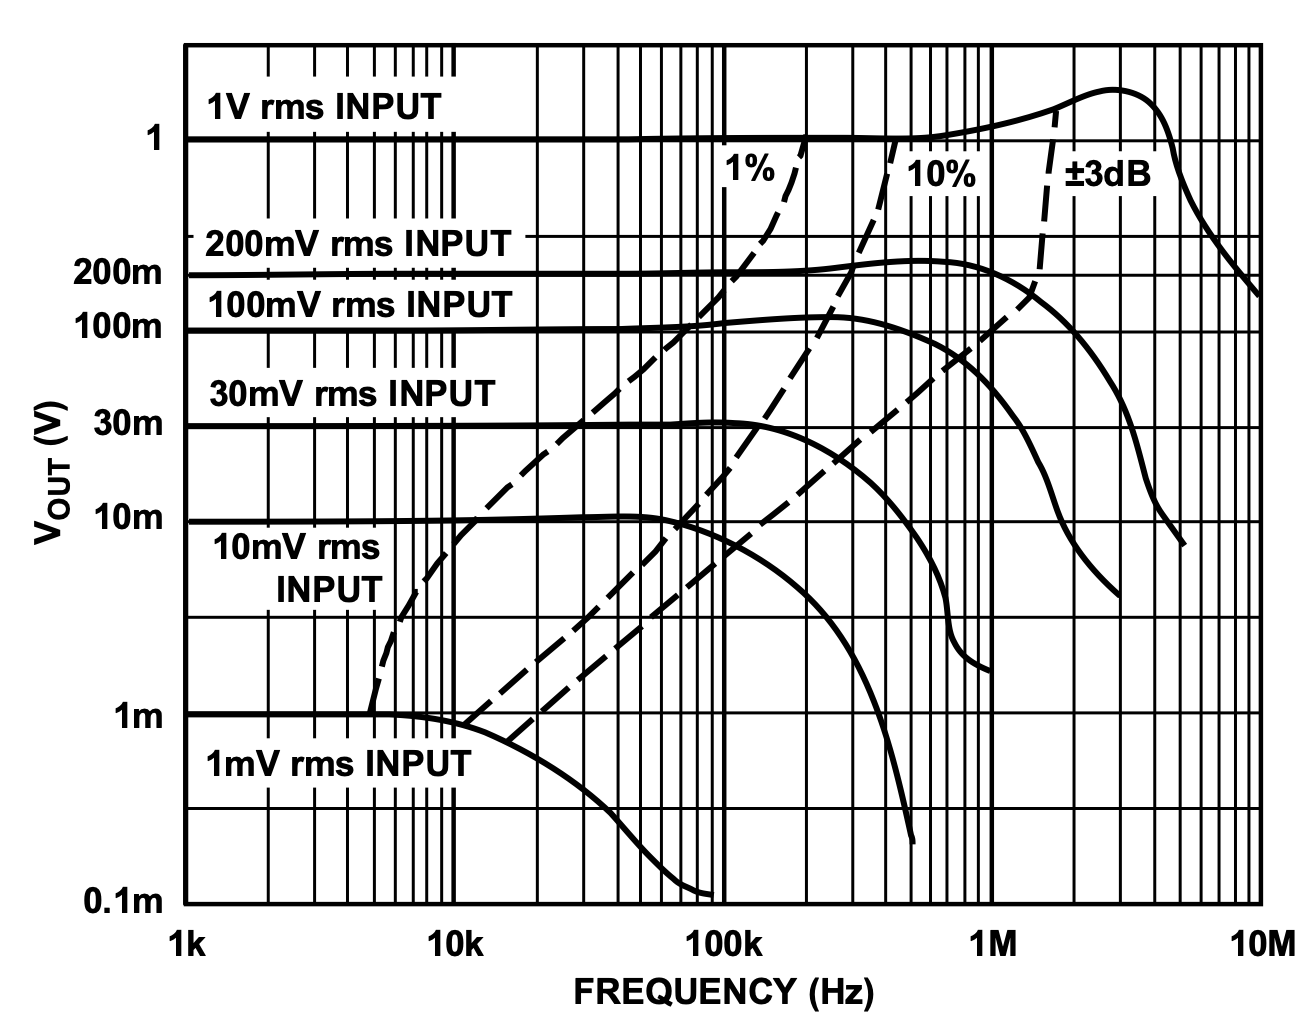
\includegraphics[width=.6\textwidth]{freq_zavisl.png}
    \caption{Závislost různých výstupních napětí na frekvenci \cite{datasheet_graf}}
    \label{datasheet}
\end{graf}
\section{Závěrečné vyhodnocení}
%Měření se mi nelíbilo, protože jsem ho nemohl provádět já.
Změřili jsme frekvenční závislost ručičkových i číslicových multimetrů. Díky frekvenčním rozsahům multimetrů jsme mohli konstatovat, který z ručních multimetrů je kvalitnější. Také jsme naměřili zajímavé chování jednoho z multimetrů a~to vyšší zobrazené napětí v určitém frekvenčním intervalu.

Nepřesnost multimetrů ve vyšších frekvencích je způsobena pravděpodobně parazitní kapacitou. Od skutečné hodnoty se nejvíce odchýlil multimetr Summit~45 a poté MY64 a to kolem frekvence 3\,kHz. Stolní multimetr HP~34401~A a ručičkový multimetr TVT-321 se začaly odchylovat až kolem frekvence 50\,kHz.


\begin{equation*}
    \mathghost \mathwitch* \mathwitch* \mathwitch* \mathghost
\end{equation*}

%--- LITERATURA a~ZDROJE (povinne) ---
\clearpage
\renewcommand{\refname}{Seznam použité literatury a~zdrojů informací} 
%\section*{Seznam použité literatury a~zdrojů informací}
\phantomsection %pridej odkaz do PDF zalozek
\addcontentsline{toc}{section}{Seznam použité literatury a~zdrojů informací}

\begin{thebibliography}{99}

%----------------------------------------------------
\subsection*{Seznam použitých internetových zdrojů}
    \bibitem{protokol} Návod k laboratorní úloze
    \bibitem{datasheet_graf} \url{https://www.analog.com/media/en/technical-documentation/data-sheets/AD636.pdf}
    \bibitem{datasheet_multimetry} \url{https://moodle.fel.cvut.cz/pluginfile.php/267148/mod_resource/content/1/Devices%20Data%20Sheets.pdf}
\end{thebibliography}



\end{document}

